\documentclass[10pt,a4paper]{article}
\usepackage[margin=2.1cm]{geometry}
\usepackage{amsmath,amssymb,bm}
\usepackage{graphicx,booktabs,caption}
\usepackage[hidelinks]{hyperref}
\usepackage{lmodern}
\usepackage[T1]{fontenc}
\usepackage{microtype}
\usepackage{xcolor}
\usepackage{enumitem}
\usepackage{tcolorbox}
\captionsetup{font=small,labelfont=bf}
\graphicspath{{../outputs/figures/}}
\newcommand{\ThermoEgap}{22.5}
\newcommand{\ThermoFgap}{2.8}
\newcommand{\ThermoSgap}{19.7}
\newcommand{\ThermoTable}{$\langle E\rangle_k-\langle E\rangle_{C1}=(22.5,\,0.0,\,9.3)$, $F_k-F_{C1}=(2.8,\,0.0,\,2.2)$ and therefore $S_k-S_{C1}=(19.7,\,0.0,\,7.1)$ for $k=$ C0, C1, C2}
\newcommand{\ShareBase}{5/86/9}
\newcommand{\dFzeroBase}{1.04}
\newcommand{\rfBase}{0.930}
\newcommand{\rCBase}{0.744}
\newcommand{\sCBase}{0.28}
\newcommand{\NLPLtestBase}{78.57}
\newcommand{\JfrobBase}{88.3}
\newcommand{\ShareMtwo}{5/83/12}
\newcommand{\dFzeroMtwo}{1.12}
\newcommand{\rfMtwo}{0.938}
\newcommand{\rCMtwo}{0.791}
\newcommand{\sCMtwo}{0.34}
\newcommand{\NLPLtestMtwo}{78.49}
\newcommand{\JfrobMtwo}{85.3}
\newcommand{\ShareNat}{14/39/47}
\newcommand{\FieldAbs}{0.95}
\newcommand{\ValBase}{81.97}
\newcommand{\EpBase}{962}
\newcommand{\ValMtwo}{82.03}
\newcommand{\EpMtwo}{962}
\newcommand{\ValCthree}{81.06}
\newcommand{\EpCthree}{791}
\newcommand{\ValCthreeQ}{80.02}
\newcommand{\EpCthreeQ}{1999}
\newcommand{\ValCthreeOne}{81.54}
\newcommand{\EpCthreeOne}{791}
\newcommand{\ValClean}{82.18}
\newcommand{\EpClean}{668}
\newcommand{\ValRepro}{82.18}
\newcommand{\EpRepro}{668}
\newcommand{\ShareClean}{5/36/59}
\newcommand{\ShareBasep}{5/86/9}
\newcommand{\NatEA}{-120.1}
\newcommand{\NatNA}{640}
\newcommand{\CeilA}{0.659}
\newcommand{\NatEB}{-135.2}
\newcommand{\NatNB}{4873}
\newcommand{\CeilB}{0.625}
\newcommand{\NatEC}{-133.3}
\newcommand{\NatNC}{1888}
\newcommand{\CeilC}{0.750}
\newcommand{\ConeALzerodist}{3.89}
\newcommand{\ConeALzeroover}{-3.47}
\newcommand{\ConeALzerorC}{0.154}
\newcommand{\ConeALzerorf}{0.683}
\newcommand{\ConeALzerohpd}{98}
\newcommand{\ConeALzeroE}{-126.3}
\newcommand{\ConeALzerodiv}{0.62}
\newcommand{\ConeALzerohit}{5}
\newcommand{\ConeALzerodtr}{0.39}
\newcommand{\ConeALQdist}{3.28}
\newcommand{\ConeALQover}{-2.96}
\newcommand{\ConeALQrC}{0.249}
\newcommand{\ConeALQrf}{0.761}
\newcommand{\ConeALQhpd}{98}
\newcommand{\ConeALQE}{-118.6}
\newcommand{\ConeALQdiv}{0.66}
\newcommand{\ConeALQhit}{18}
\newcommand{\ConeALQdtr}{0.43}
\newcommand{\ConeALonedist}{1.59}
\newcommand{\ConeALoneover}{-1.42}
\newcommand{\ConeALonerC}{0.436}
\newcommand{\ConeALonerf}{0.963}
\newcommand{\ConeALonehpd}{96}
\newcommand{\ConeALoneE}{-105.4}
\newcommand{\ConeALonediv}{0.70}
\newcommand{\ConeALonehit}{80}
\newcommand{\ConeALonedtr}{0.48}
\newcommand{\ConeALfourdist}{0.56}
\newcommand{\ConeALfourover}{-0.41}
\newcommand{\ConeALfourrC}{0.458}
\newcommand{\ConeALfourrf}{0.982}
\newcommand{\ConeALfourhpd}{96}
\newcommand{\ConeALfourE}{-106.3}
\newcommand{\ConeALfourdiv}{0.64}
\newcommand{\ConeALfourhit}{100}
\newcommand{\ConeALfourdtr}{0.46}
\newcommand{\ConeALonesixdist}{0.29}
\newcommand{\ConeALonesixover}{-0.13}
\newcommand{\ConeALonesixrC}{0.373}
\newcommand{\ConeALonesixrf}{0.969}
\newcommand{\ConeALonesixhpd}{96}
\newcommand{\ConeALonesixE}{-108.6}
\newcommand{\ConeALonesixdiv}{0.61}
\newcommand{\ConeALonesixhit}{100}
\newcommand{\ConeALonesixdtr}{0.44}
\newcommand{\ConeALsixfourdist}{0.15}
\newcommand{\ConeALsixfourover}{-0.04}
\newcommand{\ConeALsixfourrC}{0.307}
\newcommand{\ConeALsixfourrf}{0.964}
\newcommand{\ConeALsixfourhpd}{96}
\newcommand{\ConeALsixfourE}{-109.9}
\newcommand{\ConeALsixfourdiv}{0.60}
\newcommand{\ConeALsixfourhit}{100}
\newcommand{\ConeALsixfourdtr}{0.44}
\newcommand{\ConeBLzerodist}{1.51}
\newcommand{\ConeBLzeroover}{-1.34}
\newcommand{\ConeBLzerorC}{0.436}
\newcommand{\ConeBLzerorf}{0.992}
\newcommand{\ConeBLzerohpd}{99}
\newcommand{\ConeBLzeroE}{-126.6}
\newcommand{\ConeBLzerodiv}{0.62}
\newcommand{\ConeBLzerohit}{86}
\newcommand{\ConeBLzerodtr}{0.39}
\newcommand{\ConeBLQdist}{1.14}
\newcommand{\ConeBLQover}{-1.00}
\newcommand{\ConeBLQrC}{0.494}
\newcommand{\ConeBLQrf}{0.995}
\newcommand{\ConeBLQhpd}{99}
\newcommand{\ConeBLQE}{-129.0}
\newcommand{\ConeBLQdiv}{0.59}
\newcommand{\ConeBLQhit}{95}
\newcommand{\ConeBLQdtr}{0.38}
\newcommand{\ConeBLonedist}{0.86}
\newcommand{\ConeBLoneover}{-0.72}
\newcommand{\ConeBLonerC}{0.467}
\newcommand{\ConeBLonerf}{0.993}
\newcommand{\ConeBLonehpd}{99}
\newcommand{\ConeBLoneE}{-133.1}
\newcommand{\ConeBLonediv}{0.56}
\newcommand{\ConeBLonehit}{100}
\newcommand{\ConeBLonedtr}{0.36}
\newcommand{\ConeBLfourdist}{0.54}
\newcommand{\ConeBLfourover}{-0.40}
\newcommand{\ConeBLfourrC}{0.391}
\newcommand{\ConeBLfourrf}{0.986}
\newcommand{\ConeBLfourhpd}{99}
\newcommand{\ConeBLfourE}{-139.5}
\newcommand{\ConeBLfourdiv}{0.52}
\newcommand{\ConeBLfourhit}{100}
\newcommand{\ConeBLfourdtr}{0.33}
\newcommand{\ConeBLonesixdist}{0.29}
\newcommand{\ConeBLonesixover}{-0.15}
\newcommand{\ConeBLonesixrC}{0.304}
\newcommand{\ConeBLonesixrf}{0.978}
\newcommand{\ConeBLonesixhpd}{99}
\newcommand{\ConeBLonesixE}{-144.5}
\newcommand{\ConeBLonesixdiv}{0.48}
\newcommand{\ConeBLonesixhit}{100}
\newcommand{\ConeBLonesixdtr}{0.30}
\newcommand{\ConeBLsixfourdist}{0.16}
\newcommand{\ConeBLsixfourover}{-0.05}
\newcommand{\ConeBLsixfourrC}{0.262}
\newcommand{\ConeBLsixfourrf}{0.975}
\newcommand{\ConeBLsixfourhpd}{99}
\newcommand{\ConeBLsixfourE}{-146.9}
\newcommand{\ConeBLsixfourdiv}{0.47}
\newcommand{\ConeBLsixfourhit}{100}
\newcommand{\ConeBLsixfourdtr}{0.29}
\newcommand{\ConeCLzerodist}{3.28}
\newcommand{\ConeCLzeroover}{-3.06}
\newcommand{\ConeCLzerorC}{0.342}
\newcommand{\ConeCLzerorf}{0.728}
\newcommand{\ConeCLzerohpd}{98}
\newcommand{\ConeCLzeroE}{-126.5}
\newcommand{\ConeCLzerodiv}{0.62}
\newcommand{\ConeCLzerohit}{10}
\newcommand{\ConeCLzerodtr}{0.39}
\newcommand{\ConeCLQdist}{2.74}
\newcommand{\ConeCLQover}{-2.50}
\newcommand{\ConeCLQrC}{0.364}
\newcommand{\ConeCLQrf}{0.803}
\newcommand{\ConeCLQhpd}{98}
\newcommand{\ConeCLQE}{-122.4}
\newcommand{\ConeCLQdiv}{0.66}
\newcommand{\ConeCLQhit}{25}
\newcommand{\ConeCLQdtr}{0.42}
\newcommand{\ConeCLonedist}{1.05}
\newcommand{\ConeCLoneover}{-0.55}
\newcommand{\ConeCLonerC}{0.566}
\newcommand{\ConeCLonerf}{0.987}
\newcommand{\ConeCLonehpd}{98}
\newcommand{\ConeCLoneE}{-124.2}
\newcommand{\ConeCLonediv}{0.65}
\newcommand{\ConeCLonehit}{88}
\newcommand{\ConeCLonedtr}{0.44}
\newcommand{\ConeCLfourdist}{0.49}
\newcommand{\ConeCLfourover}{+0.00}
\newcommand{\ConeCLfourrC}{0.605}
\newcommand{\ConeCLfourrf}{0.993}
\newcommand{\ConeCLfourhpd}{99}
\newcommand{\ConeCLfourE}{-128.5}
\newcommand{\ConeCLfourdiv}{0.62}
\newcommand{\ConeCLfourhit}{100}
\newcommand{\ConeCLfourdtr}{0.43}
\newcommand{\ConeCLonesixdist}{0.29}
\newcommand{\ConeCLonesixover}{+0.03}
\newcommand{\ConeCLonesixrC}{0.539}
\newcommand{\ConeCLonesixrf}{0.992}
\newcommand{\ConeCLonesixhpd}{98}
\newcommand{\ConeCLonesixE}{-129.5}
\newcommand{\ConeCLonesixdiv}{0.61}
\newcommand{\ConeCLonesixhit}{100}
\newcommand{\ConeCLonesixdtr}{0.43}
\newcommand{\ConeCLsixfourdist}{0.15}
\newcommand{\ConeCLsixfourover}{+0.01}
\newcommand{\ConeCLsixfourrC}{0.509}
\newcommand{\ConeCLsixfourrf}{0.990}
\newcommand{\ConeCLsixfourhpd}{99}
\newcommand{\ConeCLsixfourE}{-129.2}
\newcommand{\ConeCLsixfourdiv}{0.61}
\newcommand{\ConeCLsixfourhit}{100}
\newcommand{\ConeCLsixfourdtr}{0.43}
\newcommand{\CthreeAsHKonedist}{0.42}
\newcommand{\CthreeAsHKoneover}{-0.14}
\newcommand{\CthreeAsHKonerC}{0.384}
\newcommand{\CthreeAsHKonerf}{0.968}
\newcommand{\CthreeAsHKonehpd}{100}
\newcommand{\CthreeAsHKoneE}{-118.4}
\newcommand{\CthreeAsHKonediv}{0.57}
\newcommand{\CthreeAsHKonehit}{100}
\newcommand{\CthreeAsHKonedtr}{0.42}
\newcommand{\CthreeAsHKtwodist}{0.91}
\newcommand{\CthreeAsHKtwoover}{+0.84}
\newcommand{\CthreeAsHKtworC}{0.219}
\newcommand{\CthreeAsHKtworf}{0.868}
\newcommand{\CthreeAsHKtwohpd}{100}
\newcommand{\CthreeAsHKtwoE}{-124.8}
\newcommand{\CthreeAsHKtwodiv}{0.45}
\newcommand{\CthreeAsHKtwohit}{100}
\newcommand{\CthreeAsHKtwodtr}{0.38}
\newcommand{\CthreeAsHKfourdist}{1.49}
\newcommand{\CthreeAsHKfourover}{+1.36}
\newcommand{\CthreeAsHKfourrC}{0.115}
\newcommand{\CthreeAsHKfourrf}{0.726}
\newcommand{\CthreeAsHKfourhpd}{100}
\newcommand{\CthreeAsHKfourE}{-120.1}
\newcommand{\CthreeAsHKfourdiv}{0.29}
\newcommand{\CthreeAsHKfourhit}{100}
\newcommand{\CthreeAsHKfourdtr}{0.39}
\newcommand{\CthreeAsHKeightdist}{1.65}
\newcommand{\CthreeAsHKeightover}{+1.47}
\newcommand{\CthreeAsHKeightrC}{0.081}
\newcommand{\CthreeAsHKeightrf}{0.635}
\newcommand{\CthreeAsHKeighthpd}{100}
\newcommand{\CthreeAsHKeightE}{-111.9}
\newcommand{\CthreeAsHKeightdiv}{0.16}
\newcommand{\CthreeAsHKeighthit}{100}
\newcommand{\CthreeAsHKeightdtr}{0.40}
\newcommand{\CthreeAsQKonedist}{0.32}
\newcommand{\CthreeAsQKoneover}{-0.04}
\newcommand{\CthreeAsQKonerC}{0.329}
\newcommand{\CthreeAsQKonerf}{0.965}
\newcommand{\CthreeAsQKonehpd}{100}
\newcommand{\CthreeAsQKoneE}{-119.2}
\newcommand{\CthreeAsQKonediv}{0.56}
\newcommand{\CthreeAsQKonehit}{100}
\newcommand{\CthreeAsQKonedtr}{0.41}
\newcommand{\CthreeAsoneKonedist}{0.74}
\newcommand{\CthreeAsoneKoneover}{-0.56}
\newcommand{\CthreeAsoneKonerC}{0.475}
\newcommand{\CthreeAsoneKonerf}{0.983}
\newcommand{\CthreeAsoneKonehpd}{100}
\newcommand{\CthreeAsoneKoneE}{-112.7}
\newcommand{\CthreeAsoneKonediv}{0.63}
\newcommand{\CthreeAsoneKonehit}{100}
\newcommand{\CthreeAsoneKonedtr}{0.45}
\newcommand{\CthreeBsHKonedist}{0.53}
\newcommand{\CthreeBsHKoneover}{-0.36}
\newcommand{\CthreeBsHKonerC}{0.402}
\newcommand{\CthreeBsHKonerf}{0.987}
\newcommand{\CthreeBsHKonehpd}{100}
\newcommand{\CthreeBsHKoneE}{-141.8}
\newcommand{\CthreeBsHKonediv}{0.52}
\newcommand{\CthreeBsHKonehit}{100}
\newcommand{\CthreeBsHKonedtr}{0.32}
\newcommand{\CthreeBsHKtwodist}{0.45}
\newcommand{\CthreeBsHKtwoover}{+0.28}
\newcommand{\CthreeBsHKtworC}{0.302}
\newcommand{\CthreeBsHKtworf}{0.960}
\newcommand{\CthreeBsHKtwohpd}{100}
\newcommand{\CthreeBsHKtwoE}{-155.6}
\newcommand{\CthreeBsHKtwodiv}{0.42}
\newcommand{\CthreeBsHKtwohit}{100}
\newcommand{\CthreeBsHKtwodtr}{0.26}
\newcommand{\CthreeBsHKfourdist}{0.89}
\newcommand{\CthreeBsHKfourover}{+0.84}
\newcommand{\CthreeBsHKfourrC}{0.184}
\newcommand{\CthreeBsHKfourrf}{0.922}
\newcommand{\CthreeBsHKfourhpd}{100}
\newcommand{\CthreeBsHKfourE}{-166.4}
\newcommand{\CthreeBsHKfourdiv}{0.31}
\newcommand{\CthreeBsHKfourhit}{100}
\newcommand{\CthreeBsHKfourdtr}{0.20}
\newcommand{\CthreeBsHKeightdist}{1.20}
\newcommand{\CthreeBsHKeightover}{+1.17}
\newcommand{\CthreeBsHKeightrC}{0.081}
\newcommand{\CthreeBsHKeightrf}{0.866}
\newcommand{\CthreeBsHKeighthpd}{100}
\newcommand{\CthreeBsHKeightE}{-168.3}
\newcommand{\CthreeBsHKeightdiv}{0.21}
\newcommand{\CthreeBsHKeighthit}{100}
\newcommand{\CthreeBsHKeightdtr}{0.17}
\newcommand{\CthreeBsQKonedist}{0.35}
\newcommand{\CthreeBsQKoneover}{-0.14}
\newcommand{\CthreeBsQKonerC}{0.338}
\newcommand{\CthreeBsQKonerf}{0.977}
\newcommand{\CthreeBsQKonehpd}{99}
\newcommand{\CthreeBsQKoneE}{-146.5}
\newcommand{\CthreeBsQKonediv}{0.48}
\newcommand{\CthreeBsQKonehit}{100}
\newcommand{\CthreeBsQKonedtr}{0.30}
\newcommand{\CthreeBsoneKonedist}{0.89}
\newcommand{\CthreeBsoneKoneover}{-0.76}
\newcommand{\CthreeBsoneKonerC}{0.483}
\newcommand{\CthreeBsoneKonerf}{0.995}
\newcommand{\CthreeBsoneKonehpd}{99}
\newcommand{\CthreeBsoneKoneE}{-133.7}
\newcommand{\CthreeBsoneKonediv}{0.56}
\newcommand{\CthreeBsoneKonehit}{100}
\newcommand{\CthreeBsoneKonedtr}{0.35}
\newcommand{\CthreeCsHKonedist}{0.49}
\newcommand{\CthreeCsHKoneover}{+0.11}
\newcommand{\CthreeCsHKonerC}{0.596}
\newcommand{\CthreeCsHKonerf}{0.994}
\newcommand{\CthreeCsHKonehpd}{100}
\newcommand{\CthreeCsHKoneE}{-129.2}
\newcommand{\CthreeCsHKonediv}{0.61}
\newcommand{\CthreeCsHKonehit}{100}
\newcommand{\CthreeCsHKonedtr}{0.42}
\newcommand{\CthreeCsHKtwodist}{1.16}
\newcommand{\CthreeCsHKtwoover}{+0.87}
\newcommand{\CthreeCsHKtworC}{0.486}
\newcommand{\CthreeCsHKtworf}{0.906}
\newcommand{\CthreeCsHKtwohpd}{98}
\newcommand{\CthreeCsHKtwoE}{-124.5}
\newcommand{\CthreeCsHKtwodiv}{0.59}
\newcommand{\CthreeCsHKtwohit}{100}
\newcommand{\CthreeCsHKtwodtr}{0.43}
\newcommand{\CthreeCsHKfourdist}{1.75}
\newcommand{\CthreeCsHKfourover}{+1.11}
\newcommand{\CthreeCsHKfourrC}{0.289}
\newcommand{\CthreeCsHKfourrf}{0.697}
\newcommand{\CthreeCsHKfourhpd}{92}
\newcommand{\CthreeCsHKfourE}{-106.5}
\newcommand{\CthreeCsHKfourdiv}{0.55}
\newcommand{\CthreeCsHKfourhit}{100}
\newcommand{\CthreeCsHKfourdtr}{0.48}
\newcommand{\CthreeCsHKeightdist}{1.79}
\newcommand{\CthreeCsHKeightover}{+1.03}
\newcommand{\CthreeCsHKeightrC}{0.122}
\newcommand{\CthreeCsHKeightrf}{0.436}
\newcommand{\CthreeCsHKeighthpd}{56}
\newcommand{\CthreeCsHKeightE}{-80.7}
\newcommand{\CthreeCsHKeightdiv}{0.40}
\newcommand{\CthreeCsHKeighthit}{100}
\newcommand{\CthreeCsHKeightdtr}{0.58}
\newcommand{\CthreeCsQKonedist}{0.38}
\newcommand{\CthreeCsQKoneover}{+0.13}
\newcommand{\CthreeCsQKonerC}{0.555}
\newcommand{\CthreeCsQKonerf}{0.991}
\newcommand{\CthreeCsQKonehpd}{99}
\newcommand{\CthreeCsQKoneE}{-132.4}
\newcommand{\CthreeCsQKonediv}{0.60}
\newcommand{\CthreeCsQKonehit}{100}
\newcommand{\CthreeCsQKonedtr}{0.42}
\newcommand{\CthreeCsoneKonedist}{0.66}
\newcommand{\CthreeCsoneKoneover}{+0.03}
\newcommand{\CthreeCsoneKonerC}{0.643}
\newcommand{\CthreeCsoneKonerf}{0.995}
\newcommand{\CthreeCsoneKonehpd}{99}
\newcommand{\CthreeCsoneKoneE}{-128.3}
\newcommand{\CthreeCsoneKonediv}{0.62}
\newcommand{\CthreeCsoneKonehit}{100}
\newcommand{\CthreeCsoneKonedtr}{0.43}


\newcommand{\PC}{\mathrm{PC}}
\newtcolorbox{keybox}{colback=black!3,colframe=black!25,boxrule=0.4pt,arc=1pt,left=5pt,right=5pt,top=3pt,bottom=3pt}

\title{\vspace{-1.2cm}Conditioning AttentionDCA on PCA coordinates, and adding fields:\\
experiments C1, C3 and M2}
\author{AttentionDCA / J-domains --- follow-up to the proposal note}
\date{\today}

\begin{document}
\maketitle

\begin{abstract}
\noindent
Three of the proposed methods are implemented and tested on the clean split:
\textbf{C1}, a harmonic restraint on the PCA coordinates added to the trained model at sampling
time; \textbf{C3}, a model with fields that depend on the target coordinates, learned by
conditional pseudo-likelihood; and \textbf{M2}, plain per-site fields added to AttentionDCA.
\S\ref{sec:sp} and \S\ref{sec:pca} are a slow refresher on the two ideas everything rests on: how an
energy function turns into sampling probabilities (and what entropy and free energy have to do
with cluster weights), and why a PCA coordinate is an exact Potts term. The results follow in
\S\ref{sec:m2}--\S\ref{sec:c3}.
\end{abstract}

%======================================================================
\section{A statistical-physics refresher}\label{sec:sp}
%======================================================================
\paragraph{Energy and probability.} A Potts model assigns every sequence $\bm x=(x_1,\dots,x_L)$
an energy $E(\bm x)$ and defines its probability by the Boltzmann distribution
\begin{equation}
p(\bm x)=\frac{e^{-\beta E(\bm x)}}{\mathcal Z},\qquad \mathcal Z=\sum_{\bm x}e^{-\beta E(\bm x)} ,
\label{eq:boltz}
\end{equation}
with $\beta=1/T$ the inverse temperature. Our model has $E(\bm x)=-\sum_i h_i(x_i)-\frac12\sum_{i\neq j}
J_{ij}(x_i,x_j)$ (the main report's model has $h=0$). The partition function $\mathcal Z$ is a sum
over $21^{63}$ sequences and is never computed; it is not needed, because everything we do uses
\emph{ratios} of probabilities, in which it cancels:
\begin{equation}
\frac{p(\bm x)}{p(\bm y)}=e^{-\beta\,[E(\bm x)-E(\bm y)]} .
\end{equation}
At $\beta=1$, a sequence one energy unit lower is $e\approx2.7$ times more probable, ten units lower
$e^{10}\approx22\,000$ times. This is why energies are quoted in \emph{nats}: an energy
difference \emph{is} a log-probability ratio.

\paragraph{How the sampler uses the energy.} One step of the sampler picks a site $i$, holds the
other $L-1$ letters fixed, and asks: what would the energy be for each of the $21$ possible letters
at $i$? It then draws letter $a$ with probability
\begin{equation}
p(x_i=a\mid\bm x_{-i})=\frac{e^{-\beta E(\bm x\text{ with }x_i=a)}}{\sum_b e^{-\beta E(\bm x\text{ with }x_i=b)}}
=\operatorname{softmax}_a\Big[\beta\Big(h_i(a)+\sum_{j\neq i}J_{ij}(a,x_j)\Big)\Big] .
\label{eq:gibbs}
\end{equation}
Only the terms touching site $i$ survive (the rest is common to all $21$ options and cancels), which
is why one update is cheap. Low-energy letters are favoured but not chosen deterministically, and
$\beta$ sets how strongly: as $\beta\to\infty$ the update always takes the best letter (a greedy
descent that freezes in a single minimum), as $\beta\to0$ it picks letters uniformly at random.
Repeating \eqref{eq:gibbs} over all sites is one \emph{sweep}. A chain started from any sequence
forgets it after a few autocorrelation times, and from then on visits each sequence a fraction of
the time equal to its Boltzmann probability \eqref{eq:boltz} --- this is detailed balance, and it is
exact when $J_{ij}(a,b)=J_{ji}(b,a)$. (Attention couplings are slightly asymmetric, so for us it holds
approximately; the main report discusses this.)

\paragraph{Why chains do not sit at the minimum: entropy.} The energy along a chain relaxes from the
starting value to a \emph{typical} value and then fluctuates around it; it does not keep going down
to the lowest-energy sequence. The reason is counting. Let $\Omega(E)$ be the number of sequences
with energy near $E$ and $S(E)=\ln\Omega(E)$ the \textbf{entropy}. The probability of finding the
chain at energy $E$ is (number of such sequences) $\times$ (probability of each):
\begin{equation}
P(E)\propto\Omega(E)\,e^{-\beta E}=e^{\,S(E)-\beta E} .
\end{equation}
Low energies are individually likely but rare; medium energies are individually less likely but
astronomically more numerous. The chain lives where $S(E)-\beta E$ is largest. Lowering the temperature
(raising $\beta$) shifts the balance towards energy, which is exactly what $\beta^*>1$ did in the main
report: it pushed the samples towards lower energy and stronger correlations.

\paragraph{From sequences to regions: free energy.} Now ask for the probability of a whole region
$k$ of sequence space, for instance a PCA cluster:
\begin{equation}
P(k)=\sum_{\bm x\in k}p(\bm x)=\frac{1}{\mathcal Z}\sum_{\bm x\in k}e^{-\beta E(\bm x)}
\equiv\frac{e^{-\beta F_k}}{\mathcal Z},
\qquad
F_k=-\frac1\beta\ln\sum_{\bm x\in k}e^{-\beta E(\bm x)} .
\label{eq:F}
\end{equation}
$F_k$ is the \textbf{free energy} of the region. It is an exact identity (take the restricted
distribution $p_k(\bm x)=e^{-\beta E(\bm x)}/e^{-\beta F_k}$ on $k$ and compute its Shannon entropy
$S_k=-\sum_{\bm x\in k}p_k\ln p_k=\beta\langle E\rangle_k-\beta F_k$) that
\begin{equation}
F_k=\langle E\rangle_k-T\,S_k ,
\label{eq:FES}
\end{equation}
the mean energy of the region minus temperature times its entropy. A region carries a large weight
if its sequences have low energy \emph{or} if there are very many of them. Mean energy alone does
not decide.

\begin{keybox}
\textbf{What $s_k$ is.} In the main report $s_k$ denotes a cluster's \textbf{share}: the fraction of
sequences (probability mass) that falls in cluster $k$, i.e.\ $s_k=P(k)$ above --- not the entropy,
which we write $S_k$. The two are related through \eqref{eq:F}--\eqref{eq:FES}: the share is
$s_k\propto e^{-\beta F_k}$, and the entropy enters through $F_k$. The free-energy error of
the model for a cluster is
\[
\Delta F_k=-\ln\frac{s_k^{\text{gen}}}{s_k^{\text{nat}}}\quad\text{nats},
\]
the amount by which the model's $F_k$ is too high (relative to the other clusters) to reproduce the
natural share. $\Delta F=1$ means the cluster gets $1/e\approx0.37$ of its natural share.
\end{keybox}

\paragraph{The entropy is visible in our data.} Applying \eqref{eq:FES} to the samples of the
baseline model gives, relative to the dominant cluster C1, \ThermoTable. The under-sampled cluster
C0 sits about \ThermoEgap\ energy units above C1 but only \ThermoFgap\ nats above it in free energy:
the difference, \ThermoSgap\ nats, is entropy. C0 is a wide, diverse basin (its sequences are also
the most mutually distant, \S\ref{sec:c1}). If energy alone set the weights, C0 would get a share
$e^{-\ThermoEgap}$ of C1's; entropy is what keeps it at a few percent.

\paragraph{How a restraint changes the picture.} Adding a term $U(\bm x)$ to the energy multiplies
every probability by $e^{-\beta U(\bm x)}$ and renormalises. With
$U=\frac{\lambda}{2}\|\PC(\bm x)-\bm t\|^2$ the factor is a Gaussian window of width $1/\sqrt{\beta\lambda}$
around the target $\bm t$: sequences far from $\bm t$ are suppressed, sequences near it keep their
relative Boltzmann weights. That is precisely a conditional distribution, which \S\ref{sec:pca}
makes explicit.

%======================================================================
\section{The PCA argument, step by step}\label{sec:pca}
%======================================================================
\paragraph{Step 1: a sequence as a vector of zeros and ones.} PCA works on numbers, so each
sequence is first one-hot encoded: for every site $i$ and letter $a$ there is an entry
$x_{ia}\in\{0,1\}$, equal to $1$ iff site $i$ carries letter $a$. A sequence becomes a vector of
length $Lq=63\times21=1323$ with exactly one $1$ per site. Toy example with $L=3$ and a two-letter
alphabet $\{\mathrm A,\mathrm G\}$:
\[
\mathrm{AGA}\;\mapsto\;(\underbrace{1,0}_{\text{site 1}}\,|\,\underbrace{0,1}_{\text{site 2}}\,|\,
\underbrace{1,0}_{\text{site 3}}).
\]

\paragraph{Step 2: a PCA coordinate is a dot product.} Fitting PCA finds directions $\bm v_c$ (unit
vectors of length $1323$) along which the natural sequences vary most. Fitting is a nonlinear
procedure, but once it is done, the coordinate of a sequence is just its projection on $\bm v_c$:
\begin{equation}
\PC_c(\bm x)=\bm v_c\cdot(\bm x-\bm\mu)=\sum_{i,a}v_{c,ia}\,x_{ia}-m_c,\qquad m_c=\bm v_c\cdot\bm\mu ,
\end{equation}
with $\bm\mu$ the mean one-hot vector. This is linear in $\bm x$; nothing is approximated.

\paragraph{Step 3: because $\bm x$ is one-hot, the dot product is a table lookup per site.} At each
site exactly one $x_{ia}$ is $1$, so the sum over $a$ picks one number per site:
\begin{equation}
\PC_c(\bm x)=\sum_{i=1}^{L}V_c(i,x_i)-m_c ,\qquad V_c(i,a)\equiv v_{c,ia}.
\label{eq:lookup}
\end{equation}
In the toy example with $\bm v=(0.5,-0.5\,|\,0.1,0.3\,|\,{-0.2},0.4)$, $\PC(\mathrm{AGA})=0.5+0.3-0.2-m$,
and mutating site 3 from A to G moves the coordinate by $0.4-(-0.2)=+0.6$, whatever the other sites
are. The coordinate is a \emph{score table}, like a position-specific scoring matrix: every site adds a
contribution depending only on its own letter. For the J-domains a single substitution moves
$\PC_1$ by $0.125$ on average, while the family spans about $6.9$ units of $\PC_1$ (standard deviation $2.06$); going from one cluster to
another takes tens of coordinated substitutions.

\paragraph{Step 4: the square of a sum of site terms is a Potts energy.} A Potts energy is built from
site terms ($h_i(x_i)$) and pair terms ($J_{ij}(x_i,x_j)$). Write $u_i=V_c(i,x_i)$ and expand
\[
\Big(\sum_i u_i-m_c-t_c\Big)^2=\underbrace{\sum_{i\neq j}u_iu_j}_{\text{pairs}}
+\underbrace{\sum_iu_i^2-2(m_c+t_c)\sum_iu_i}_{\text{sites}}+\text{const}.
\]
So the restraint $\frac{\lambda}{2}\sum_c(\PC_c(\bm x)-t_c)^2$ is exactly a Potts energy with
\begin{equation}
\Delta J_{ij}(a,b)=-\lambda\sum_cV_c(i,a)V_c(j,b),\qquad
\Delta h_i(a)=\lambda\sum_c\big[(m_c+t_c)V_c(i,a)-\tfrac12V_c(i,a)^2\big].
\label{eq:dJdh}
\end{equation}
Adding it to the learned energy gives \emph{another Potts model}. The sampler is unchanged except
that each site update also scores, for each candidate letter, how far the resulting coordinate
would be from the target --- a lookup in \eqref{eq:lookup}. Nothing is learned. (Unit test: on a toy
system the sampler reproduces the enumerated distribution $\propto e^{-E-\lambda\|\PC-\bm t\|^2/2}$,
and \eqref{eq:dJdh} matches the direct restraint to $10^{-10}$.)

\paragraph{Step 5: what $\lambda$ means --- a noisy measurement.} By Bayes' rule, if we ``measure''
the coordinate of a sequence with Gaussian noise of width $\sigma$ and obtain $\bm t$, the posterior
over sequences is
\begin{equation}
p(\bm x\mid\bm t)\;\propto\;p(\bm x)\;e^{-\|\PC(\bm x)-\bm t\|^2/2\sigma^2} ,
\label{eq:bayes}
\end{equation}
which is the restrained Boltzmann distribution with $\lambda=1/\sigma^2$ (at $\beta=1$). So
$\lambda$ is not a fudge factor: $1/\sqrt\lambda$ is the width of the target region, and
$\lambda\to\infty$ is the exact conditional $p(\bm x\mid\PC(\bm x)=\bm t)$. The old appended-label
model tried to \emph{learn} this relationship from data; here it is written down.

\paragraph{Step 6: why it cannot blow up the protein in the old way.} The restraint only involves
the two directions $\bm v_1,\bm v_2$. Everything else about the sequence --- which residues are
conserved, which pairs co-vary, the HPD motif --- is still scored by the learned $E(\bm x)$ alone.
Raising $\lambda$ narrows the window; it never amplifies the learned couplings. The price of a
large $\lambda$ is different: the chain must satisfy the coordinate almost exactly and may accept
worse energies to do so. That trade-off is what the experiments measure.

\paragraph{Step 7: what C3 learns, in this language.} C3 is trained on pairs (sequence, its
coordinate plus noise of width $\sigma$), so the conditional it is fitted to is exactly
\eqref{eq:bayes} with $\lambda=1/\sigma^2$. Expanding as in \eqref{eq:dJdh}, that distribution has
(i) a coupling correction $-\lambda\sum_cV_cV_c$ that does \emph{not} depend on $\bm t$, and (ii) a
field that is \emph{linear} in $\bm t$. C3's parametrisation --- shared couplings plus fields
$h_i(a\mid\bm z)=\sum_f W_f(i,a)\phi_f(\bm z)$ with $\phi$ containing $1,z_1,z_2$ --- can therefore
represent it: the learned $J$ absorbs part (i), the linear features carry part (ii). We train C3 at
$\sigma=1,\,0.5,\,0.25$ and compare it with C1 at the matching $\lambda=1,4,16$. This also predicts
what happens if the $\bm z$-dependent field is amplified by a gain $\kappa>1$ at sampling time,
which is the analogue of the old $\beta_\mathrm{PCA}$: the field part (ii) grows but the
coupling part (i), which acts as the spring holding $\PC$ \emph{at} the target, does not.
Sequences are then pushed \emph{past} the target --- the ``shifted too far right'' of the previous
study. \S\ref{sec:c3} tests this prediction.

%======================================================================
\section{Setup}\label{sec:setup}
%======================================================================
All models are trained on the clean split with the main report's architecture and hyper-parameters
($H=128$, $d=10$, $\lambda_J=10^{-3}$, same seed and batches), and early stopping with a patience of
$150$ epochs; the only differences between runs are the field terms. Fields carry an $L_2$ penalty
$10^{-4}\|W\|^2$.
\begin{description}[leftmargin=1.2em,itemsep=1pt]
\item[Baseline] field-free AttentionDCA (best epoch \EpBase, validation NLPL \ValBase).
\item[M2] $+$ per-site fields $h_i(a)$, learned jointly (\ValMtwo).
\item[C1] the baseline plus the restraint \eqref{eq:dJdh} at sampling time; nothing is retrained.
      $\lambda\in\{0.25,1,4,16,64\}$.
\item[C3] fields $h_i(a\mid\bm z)=\sum_fW_f(i,a)\phi_f(\bm u)$, $\phi=(1,u_1,u_2,u_1^2,u_2^2,u_1u_2)$,
      $\bm u$ the standardised coordinates, trained on $(\bm x,\PC(\bm x)+\sigma\bm\epsilon)$ with fresh
      noise at every batch, for $\sigma=1,\,0.5,\,0.25$ (validation NLPL \ValCthreeOne, \ValCthree,
      \ValCthreeQ, scored with the noiseless coordinate). At sampling time $\bm z=\bm t$; a gain
      $\kappa$ optionally multiplies the $\bm z$-dependent part of the field.
\end{description}
\textbf{Targets} are the three k-means centres of the main report (C0 = the under-sampled HscB-like
cluster, C1, C2). For each method, target and setting, $3000$ chains start from random
\emph{training} sequences --- mostly in another cluster, so they have to travel --- and run $500$
sweeps. The restrained chains converge within $50$ sweeps for $\lambda\ge4$ and $\sim100$ for
$\lambda=1$ (figure in the appendix). The PCA frame is the one used in every figure of the main
report (fitted on the test set); it is a fixed linear map, $V$ and $\bm m$ are just constants.

\textbf{Metrics}, all against the natural \emph{test} sequences of the target cluster
(\NatNA, \NatNB, \NatNC\ sequences for C0, C1, C2; reweighted):
distance $\|\PC-\bm t\|$; \emph{overshoot}, the signed miss along the line from the family centre to
the target ($>0$: beyond the target, $<0$: stopped short); share landing in the target cluster;
$r(f_i)$ and $r(C_{ij})$; HPD motif retained (columns 28--30, present in $\ge99\%$ of natural
sequences); mean energy under one common judge (the baseline model, so C1 and C3 are on the same
scale; natural cluster means \NatEA, \NatEB, \NatEC); mean distance to the closest training
sequence ($d_\text{train}$, novelty) and mean pairwise distance within the pool (div., diversity).
Because $C_{ij}$ estimates are noisy, \emph{every} pool is evaluated at the same size, $3000$; the
natural ceiling is a weight-proportional draw of $3000$ training sequences of the cluster. With
these sizes the ceiling is $r(C_{ij})=\CeilA$, \CeilB, \CeilC\ --- lower than the full-family
values of the main report simply because a cluster has fewer sequences.

%======================================================================
\section{M2: explicit fields}\label{sec:m2}
%======================================================================
\begin{table}[h]\centering\small
\begin{tabular}{lcccccc}
\toprule
 & val.\ NLPL & test NLPL & $r(f_i)$ & $r(C_{ij})$ / slope & shares C0/C1/C2 (\%) & $\Delta F_{C0}$ \\
\midrule
natural & -- & -- & -- & -- & 14/39/47 & -- \\
no fields & 81.97 & 78.57 & 0.930 & 0.744 / 0.28 & 5/86/9 & 1.04 \\
M2 (+ fields) & 82.03 & 78.49 & 0.938 & 0.791 / 0.34 & 5/83/12 & 1.12 \\
\bottomrule
\end{tabular}

\caption{Fields versus no fields, same training protocol. NLPL in nats per sequence; $r$ and slope of
the generated statistics against the natural test set (full family); shares by nearest cluster
centre; $\Delta F_{C0}=-\ln(s^\text{gen}_{C0}/s^\text{nat}_{C0})$.}
\label{tab:m2}
\end{table}

\paragraph{Fields are learned, but they replace couplings rather than add information.} The fields
are far from zero (mean $|h_i(a)|=\FieldAbs$) and the coupling norm drops from \JfrobBase\ to
\JfrobMtwo, yet the pseudo-likelihood is unchanged (Table~\ref{tab:m2}: validation \ValBase\ vs
\ValMtwo, test \NLPLtestBase\ vs \NLPLtestMtwo). This confirms the premise of AttentionDCA: the
conserved-residue and gap columns of the value matrices $V^h$ already act as fields. The generated
statistics improve modestly ($r(f_i)$ \rfBase$\to$\rfMtwo, $r(C_{ij})$ \rCBase$\to$\rCMtwo), so fields
are a cheap, harmless addition.

\paragraph{Fields do not fix the missing cluster.} C0 receives $5\%$ of the samples with and without
fields ($\Delta F_{C0}=\dFzeroBase\to\dFzeroMtwo$). Figure~\ref{fig:m2} (right) shows why, using the
decomposition $F=\langle E\rangle-S$ of \S\ref{sec:sp}. In both models C0 lies about $20$ energy units
above C1 and $17$--$20$ nats higher in entropy; the two nearly cancel and leave a free-energy
difference of $2.8$--$2.9$ nats. A field shifts the energy of every sequence carrying a given
residue; it cannot, by itself, rebalance two basins whose weights are set by a near-cancellation
between energy and entropy. That balance is not what pseudo-likelihood measures --- it fits each
site's conditional given the rest of the sequence, never the relative mass of whole basins.

\begin{figure}[t]\centering
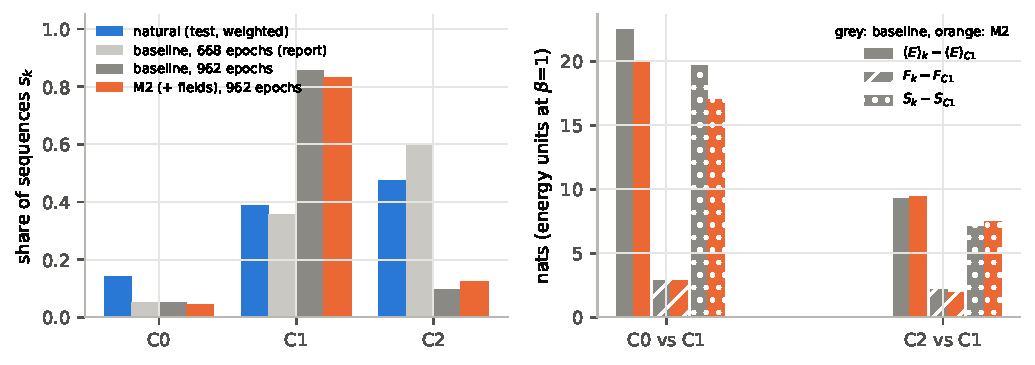
\includegraphics[width=0.92\textwidth]{m2_shares.pdf}
\caption{Left: cluster shares. The two grey bars (light, dark) are the \emph{same} field-free model at two
training lengths. Right: per-cluster mean energy, free energy and entropy of each model's own
samples, relative to C1 ($F_k=-\ln s_k$, $S_k=\langle E\rangle_k-F_k$, $\beta=1$).}
\label{fig:m2}
\end{figure}

\paragraph{A finding worth more than M2 itself: the mode weights depend on when training stops.}
The main report's model stopped at epoch \EpClean\ (patience 50); retraining it with the current code
reproduces its couplings bit for bit. The same run continued to epoch \EpBase\ (patience 150) has a
\emph{better} validation pseudo-likelihood (\ValClean$\to$\ValBase, $0.2$ nats per sequence) and
the same C0 deficit, but its C1/C2 balance has flipped: shares C0/C1/C2 go from \ShareClean\ to
\ShareBasep\ (natural \ShareNat). That is a $2.7$-nat swing in the relative free energy of C1 and C2
for $0.2$ nats of pseudo-likelihood --- and it makes the longer-trained model a \emph{worse}
generator of the family ($r(C_{ij})=\rCBase$, slope \sCBase, against $0.87$ for the report's model),
because full-family correlations are dominated by the contrast between clusters. Two consequences:
(i) the main report's statement that C1 and C2 are ``covered'' is true of that checkpoint but is not
a robust property of the method; the C0 deficit, by contrast, is present in every model trained;
(ii) the validation pseudo-likelihood cannot select a model for its sampling behaviour. Fixing the
mode weights needs an objective that sees them (M4, likelihood/PCD fine-tuning) or, as below, an
explicit choice of where to sample.

%======================================================================
\section{C1: the analytic restraint}\label{sec:c1}
%======================================================================
\begin{figure}[t]\centering
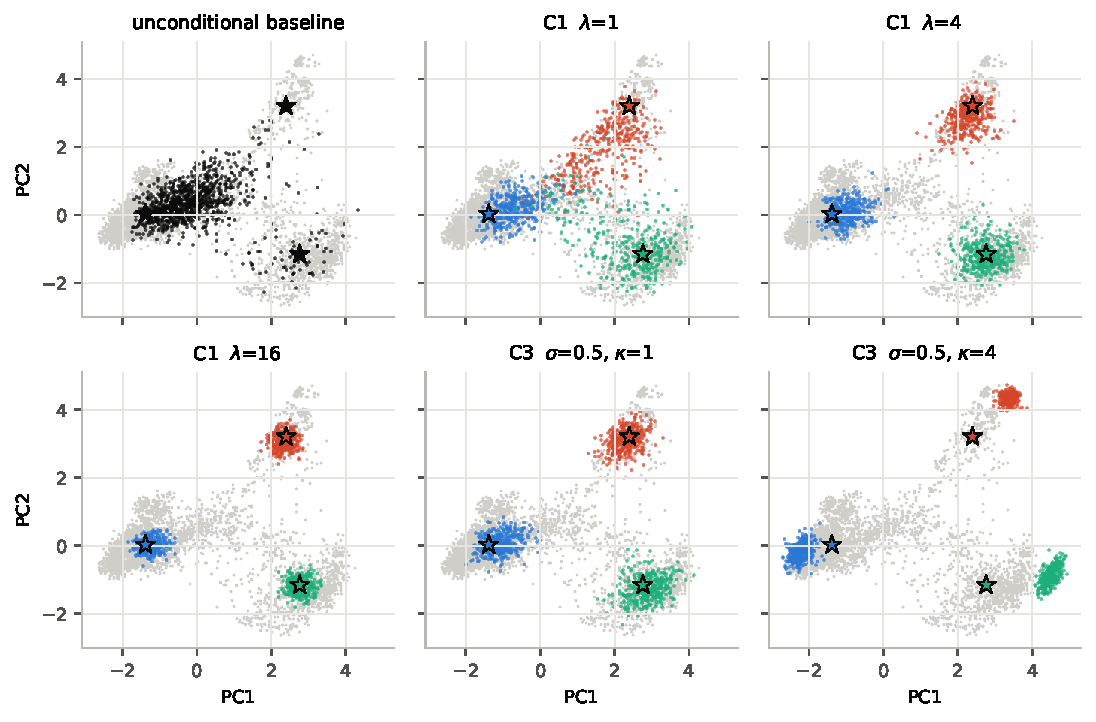
\includegraphics[width=0.86\textwidth]{cond_pca.pdf}
\caption{Samples in the PCA plane (grey: natural test). Stars: targets C0 (red), C1 (blue), C2
(green); points are coloured by the target they were aimed at. Top left: the unconditional baseline,
which visits C1 almost exclusively. Bottom right: C3 with its target field amplified by $\kappa=4$ ---
every pool lands \emph{beyond} its target.}
\label{fig:pca}
\end{figure}

\begin{figure}[t]\centering
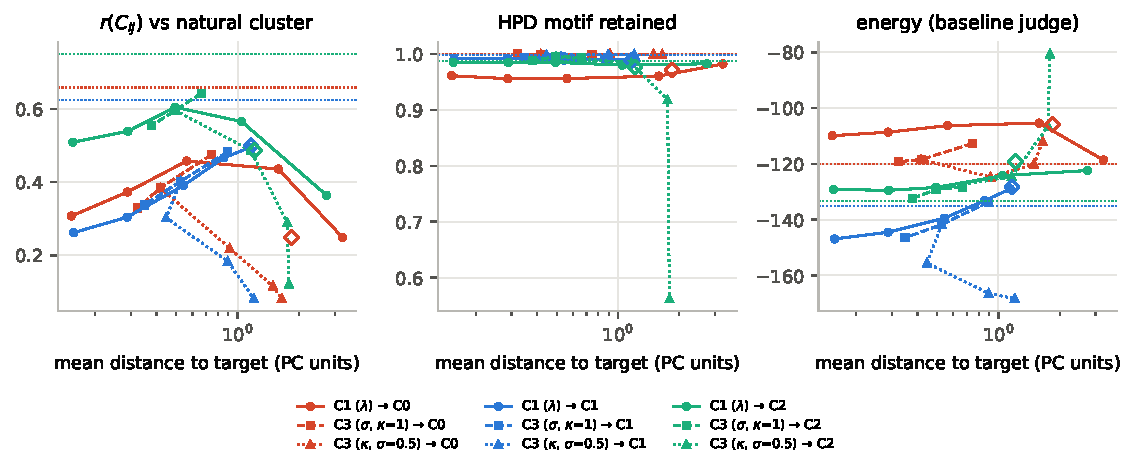
\includegraphics[width=\textwidth]{cond_tradeoff.pdf}
\caption{Accuracy--quality trade-off, one curve per method and target (colour). Solid circles: C1,
$\lambda=0.25\to64$ (right to left). Dashed squares: C3 at $\kappa=1$, $\sigma=1\to0.25$. Dotted
triangles: C3, $\sigma=0.5$, $\kappa=1\to8$. Open diamonds: rejection from the unconditional
baseline. Dotted horizontal lines: natural ceiling ($r(C_{ij})$) and natural cluster value (HPD,
energy).}
\label{fig:trade}
\end{figure}

\paragraph{It steers, to any target, including the one the model neglects.} Without restraint,
$5\%$, $86\%$ and $10\%$ of the chains end in C0, C1, C2. From $\lambda=4$ on, $100\%$ end in the
cluster they are aimed at (Figure~\ref{fig:pca}), and the mean distance to the target falls as
$1/\sqrt\lambda$ --- $0.5$, $0.3$, $0.15$ at $\lambda=4,16,64$, the width of the Gaussian window
of \S\ref{sec:pca}, Step~5. The response is monotone in $\lambda$, unlike $\beta_\mathrm{PCA}$ in the
previous study.

\paragraph{It keeps the protein.} The HPD motif is retained in $96$--$99\%$ of the samples at every
$\lambda$ (Tables~\ref{tab:C0}--\ref{tab:C2}), against $99$--$100\%$ for the natural clusters;
$r(f_i)$ against the target cluster's natural sequences is $0.96$--$0.99$ for $\lambda\ge1$.
The covariation agreement $r(C_{ij})$ \emph{peaks} at a moderate stiffness --- \ConeALfourrC\ for C0
and $0.605$ for C2 at $\lambda=4$, $0.49$ for C1 at $\lambda=0.25$ --- against ceilings \CeilA,
\CeilB, \CeilC, and declines for larger $\lambda$. Most of that decline is not damage but a mismatch
of scale: a natural cluster has a radius of about one PC unit, so a window of width $0.15$ samples
the \emph{centre} of the cluster rather than the cluster, and the pool loses the cluster's internal
variation (diversity drops from $0.56$ to $0.47$ for C1). \textbf{The useful regime is
$\lambda\approx1$--$4$}, a window comparable to the size of the region one wants.

\paragraph{Against rejection, the exact conditional.} Keeping only the unconditional samples that
fall in C0 gives $496$ sequences out of $10\,000$; at the same cost C1 produces $10\,000$. Where the
two can be compared they agree on what the model believes: C1 at $\lambda=4$ and rejection give C0
sequences of the same energy (\ConeALfourE\ vs $-106.0$), as they should if C1 samples the model's
own conditional. That energy is $14$ units above the natural C0 sequences (\NatEA): the model's C0
basin is not only under-weighted (\S\ref{sec:m2}) but also displaced towards higher energy, and C1,
which only restrains the coordinates, inherits it faithfully.

\paragraph{It inherits the prior's error at weak restraint.} The overshoot column is negative at
small $\lambda$: chains stop short of the target, on the side of the family centre ($-1.42$ for C0
at $\lambda=1$, where only $80\%$ reach the cluster). The restraint has to overcome the model's own
free-energy penalty on C0, so the weaker it is, the more the model's mis-weighting shows through.

%======================================================================
\section{C3: the learned conditional field}\label{sec:c3}
%======================================================================
\paragraph{At its natural setting it matches C1.} Knowing the coordinate improves the conditional
pseudo-likelihood by $0.4$, $0.9$ and $2.0$ nats for $\sigma=1,\,0.5,\,0.25$: the sharper the
coordinate, the more it says about each site. Sampled at $\bm z=\bm t$ with $\kappa=1$, C3 lands on
target with the accuracy of C1 at the matching $\lambda=1/\sigma^2$ (dashed vs solid curves of
Figure~\ref{fig:trade}; distances \CthreeAsHKonedist, $0.53$, $0.49$ at $\sigma=0.5$ against $0.56$,
$0.54$, $0.49$ for C1 at $\lambda=4$) and with comparable quality (HPD $99$--$100\%$,
$r(C_{ij})$ within $0.07$ of C1 for every target). This is the prediction of \S\ref{sec:pca}, Step 7: C3,
trained on noisy coordinates, learns the same distribution that C1 writes down.

\paragraph{Where it is better: the neglected cluster.} The one systematic difference is C0. C3 gets
closer to it at weak conditioning ($\sigma=1$: distance $0.74$, overshoot $-0.56$, against $1.59$
and $-1.42$ for C1 at $\lambda=1$), and its C0 sequences have lower energy (\CthreeAsHKoneE\ at
$\sigma=0.5$ against \ConeALfourE), closer to the natural C0 (\NatEA). The reason is the prior. C1
multiplies the \emph{unconditional} model, with its C0 free-energy error, by a window; C3 was trained
on (sequence, coordinate) pairs and learned the conditional directly from data, so it does not
inherit that error. This is the one place where a learned conditional earns its extra parameters
for a sequence-derived label.

\paragraph{Amplifying the target field reproduces the old failure, exactly as predicted.} With the
gain $\kappa$ on the $\bm z$-dependent field the samples \emph{overshoot}: $+0.84$, $+1.36$,
$+1.47$ for C0 and $+0.28$, $+0.84$, $+1.17$ for C1 at $\kappa=2,4,8$ (Figure~\ref{fig:pca}, bottom
right). Everything else degrades with it: diversity collapses to $0.16$ (C0) and $0.21$ (C1) ---
near-copies of one sequence --- $r(C_{ij})$ falls to $0.08$--$0.12$, and for C2 the HPD motif is lost
in $44\%$ of the samples while the energy rises to $-81$, $50$ units above the natural cluster. The
mechanism is the one derived in Step 7: $\kappa$ amplifies the field that pushes towards the target
but not the coupling term that holds the coordinate \emph{at} the target. This is the
$\beta_\mathrm{PCA}$ pathology of the previous study --- ``shifts too far right, loses the HPD
motif'' --- now reproduced on demand and explained.

%======================================================================
\section{Summary}\label{sec:sum}
%======================================================================
\begin{itemize}[leftmargin=*,itemsep=2pt]
\item \textbf{C1 works and needs no training.} Monotone control by $\lambda$, all three clusters
      reachable (C0 from $5\%$ to $100\%$), HPD kept, best covariation agreement at
      $\lambda\approx1$--$4$. It samples the model's own conditional, so it inherits the model's
      errors about a region (C0 is reached, but at too high an energy).
\item \textbf{C3 matches C1 at $\lambda=1/\sigma^2$} and is better on the neglected cluster because
      it learns the conditional from data instead of reweighting a biased prior. Use it at $\kappa=1$;
      amplifying it reproduces the old over-steering pathology.
\item \textbf{M2} leaves the pseudo-likelihood unchanged, slightly improves the generated
      statistics, and does not fix the mode weights.
\item \textbf{Mode weights are fragile under pseudo-likelihood}: $294$ more epochs moved the C1/C2
      balance by $2.7$ nats for a $0.2$-nat gain in validation PL, while C0 stayed at $5\%$ in every
      model.
\end{itemize}

\noindent\textbf{Next step suggested by these results.} Conditioning gives a direct, cheap fix for
the mode weights: draw a target $\bm t$ from the natural distribution of coordinates (the reweighted
training PCA points), then sample $\bm x\sim p(\bm x\mid\bm t)$ with C3 at $\kappa=1$ (or C1 at
$\lambda\approx4$). This is ancestral sampling of $p(\bm t)\,p(\bm x\mid\bm t)$: the cluster shares
are the natural ones \emph{by construction}, and the within-cluster statistics are those measured
here. It would remove both the C0 deficit and the training-length dependence of the C1/C2 balance
without retraining anything but C3.

\appendix
\section{Per-target tables and convergence}
\noindent Columns: mean distance to target; overshoot (signed, $>0$ beyond the target); \% landing in
the target cluster; $r(f_i)$, $r(C_{ij})$ against the natural test sequences of the cluster; \% with
the HPD motif; mean energy under the baseline judge; mean distance to the closest training
sequence; mean pairwise distance in the pool. All pools of size $3000$ except the rejection pool.

\begin{table}[h]\centering\scriptsize\setlength{\tabcolsep}{4pt}
\begin{tabular}{lccccccccc}
\toprule
 & dist. & overshoot & in $C_k$ (\%) & $r(f_i)$ & $r(C_{ij})$ & HPD (\%) & $E$ & $d_\text{train}$ & div. \\
\midrule
natural (train, ceiling) & 0.99 & -0.75 & 100 & 0.994 & 0.659 & 100 & -123.3 & 0.00 & 0.67 \\
rejection from baseline (n=496) & 1.84 & -1.70 & 100 & 0.928 & 0.248 & 97 & -106.0 & 0.49 & 0.69 \\
unconditional baseline & 3.89 & -3.47 & 5 & 0.684 & 0.158 & 99 & -126.3 & 0.39 & 0.62 \\
\midrule
C1 $\lambda{=}1$ & 1.59 & -1.42 & 80 & 0.963 & 0.436 & 96 & -105.4 & 0.48 & 0.70 \\
C1 $\lambda{=}4$ & 0.56 & -0.41 & 100 & 0.982 & 0.458 & 96 & -106.3 & 0.46 & 0.64 \\
C1 $\lambda{=}16$ & 0.29 & -0.13 & 100 & 0.969 & 0.373 & 96 & -108.6 & 0.44 & 0.61 \\
C1 $\lambda{=}64$ & 0.15 & -0.04 & 100 & 0.964 & 0.307 & 96 & -109.9 & 0.44 & 0.60 \\
\midrule
C3 $\sigma{=}1$ & 0.74 & -0.56 & 100 & 0.983 & 0.475 & 100 & -112.7 & 0.45 & 0.63 \\
C3 $\sigma{=}0.5$ & 0.42 & -0.14 & 100 & 0.968 & 0.384 & 100 & -118.4 & 0.42 & 0.57 \\
C3 $\sigma{=}0.25$ & 0.32 & -0.04 & 100 & 0.965 & 0.329 & 100 & -119.2 & 0.41 & 0.56 \\
C3 $\sigma{=}0.5$, $\kappa{=}2$ & 0.91 & +0.84 & 100 & 0.868 & 0.219 & 100 & -124.8 & 0.38 & 0.45 \\
C3 $\sigma{=}0.5$, $\kappa{=}4$ & 1.49 & +1.36 & 100 & 0.726 & 0.115 & 100 & -120.1 & 0.39 & 0.29 \\
C3 $\sigma{=}0.5$, $\kappa{=}8$ & 1.65 & +1.47 & 100 & 0.635 & 0.081 & 100 & -111.9 & 0.40 & 0.16 \\
\bottomrule
\end{tabular}

\caption{Target C0 (the under-sampled cluster). Natural test energy \NatEA.}\label{tab:C0}
\end{table}
\begin{table}[h]\centering\scriptsize\setlength{\tabcolsep}{4pt}
\begin{tabular}{lccccccccc}
\toprule
 & dist. & overshoot & in $C_k$ (\%) & $r(f_i)$ & $r(C_{ij})$ & HPD (\%) & $E$ & $d_\text{train}$ & div. \\
\midrule
natural (train, ceiling) & 1.30 & -1.16 & 100 & 0.996 & 0.625 & 100 & -136.0 & 0.00 & 0.60 \\
rejection from baseline (n=3000) & 1.17 & -1.02 & 100 & 0.995 & 0.500 & 99 & -128.3 & 0.38 & 0.59 \\
unconditional baseline & 1.52 & -1.36 & 86 & 0.992 & 0.425 & 99 & -126.2 & 0.39 & 0.62 \\
\midrule
C1 $\lambda{=}1$ & 0.86 & -0.72 & 100 & 0.993 & 0.467 & 99 & -133.1 & 0.36 & 0.56 \\
C1 $\lambda{=}4$ & 0.54 & -0.40 & 100 & 0.986 & 0.391 & 99 & -139.5 & 0.33 & 0.52 \\
C1 $\lambda{=}16$ & 0.29 & -0.15 & 100 & 0.978 & 0.304 & 99 & -144.5 & 0.30 & 0.48 \\
C1 $\lambda{=}64$ & 0.16 & -0.05 & 100 & 0.975 & 0.262 & 99 & -146.9 & 0.29 & 0.47 \\
\midrule
C3 $\sigma{=}1$ & 0.89 & -0.76 & 100 & 0.995 & 0.483 & 99 & -133.7 & 0.35 & 0.56 \\
C3 $\sigma{=}0.5$ & 0.53 & -0.36 & 100 & 0.987 & 0.402 & 100 & -141.8 & 0.32 & 0.52 \\
C3 $\sigma{=}0.25$ & 0.35 & -0.14 & 100 & 0.977 & 0.338 & 99 & -146.5 & 0.30 & 0.48 \\
C3 $\sigma{=}0.5$, $\kappa{=}2$ & 0.45 & +0.28 & 100 & 0.960 & 0.302 & 100 & -155.6 & 0.26 & 0.42 \\
C3 $\sigma{=}0.5$, $\kappa{=}4$ & 0.89 & +0.84 & 100 & 0.922 & 0.184 & 100 & -166.4 & 0.20 & 0.31 \\
C3 $\sigma{=}0.5$, $\kappa{=}8$ & 1.20 & +1.17 & 100 & 0.866 & 0.081 & 100 & -168.3 & 0.17 & 0.21 \\
\bottomrule
\end{tabular}

\caption{Target C1. Natural test energy \NatEB.}\label{tab:C1}
\end{table}
\begin{table}[h]\centering\scriptsize\setlength{\tabcolsep}{4pt}
\begin{tabular}{lccccccccc}
\toprule
 & dist. & overshoot & in $C_k$ (\%) & $r(f_i)$ & $r(C_{ij})$ & HPD (\%) & $E$ & $d_\text{train}$ & div. \\
\midrule
natural (train, ceiling) & 0.83 & -0.08 & 100 & 0.997 & 0.750 & 99 & -137.3 & 0.00 & 0.64 \\
rejection from baseline (n=948) & 1.21 & -0.74 & 100 & 0.977 & 0.487 & 98 & -119.2 & 0.45 & 0.68 \\
unconditional baseline & 3.29 & -3.07 & 10 & 0.729 & 0.336 & 99 & -127.2 & 0.39 & 0.62 \\
\midrule
C1 $\lambda{=}1$ & 1.05 & -0.55 & 88 & 0.987 & 0.566 & 98 & -124.2 & 0.44 & 0.65 \\
C1 $\lambda{=}4$ & 0.49 & +0.00 & 100 & 0.993 & 0.605 & 99 & -128.5 & 0.43 & 0.62 \\
C1 $\lambda{=}16$ & 0.29 & +0.03 & 100 & 0.992 & 0.539 & 98 & -129.5 & 0.43 & 0.61 \\
C1 $\lambda{=}64$ & 0.15 & +0.01 & 100 & 0.990 & 0.509 & 99 & -129.2 & 0.43 & 0.61 \\
\midrule
C3 $\sigma{=}1$ & 0.66 & +0.03 & 100 & 0.995 & 0.643 & 99 & -128.3 & 0.43 & 0.62 \\
C3 $\sigma{=}0.5$ & 0.49 & +0.11 & 100 & 0.994 & 0.596 & 100 & -129.2 & 0.42 & 0.61 \\
C3 $\sigma{=}0.25$ & 0.38 & +0.13 & 100 & 0.991 & 0.555 & 99 & -132.4 & 0.42 & 0.60 \\
C3 $\sigma{=}0.5$, $\kappa{=}2$ & 1.16 & +0.87 & 100 & 0.906 & 0.486 & 98 & -124.5 & 0.43 & 0.59 \\
C3 $\sigma{=}0.5$, $\kappa{=}4$ & 1.75 & +1.11 & 100 & 0.697 & 0.289 & 92 & -106.5 & 0.48 & 0.55 \\
C3 $\sigma{=}0.5$, $\kappa{=}8$ & 1.79 & +1.03 & 100 & 0.436 & 0.122 & 56 & -80.7 & 0.58 & 0.40 \\
\bottomrule
\end{tabular}

\caption{Target C2. Natural test energy \NatEC.}\label{tab:C2}
\end{table}
\begin{figure}[h]\centering
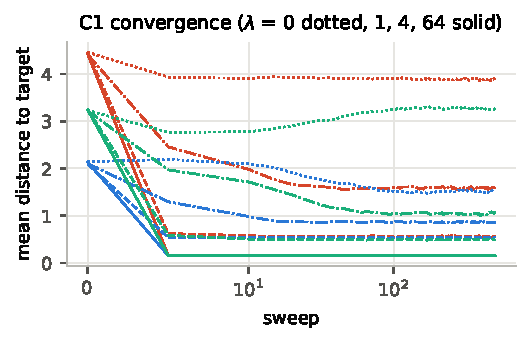
\includegraphics[width=0.48\textwidth]{cond_convergence.pdf}
\caption{C1: mean distance to the target along the chains (colour = target, line style = $\lambda$).}
\end{figure}


\end{document}
